\textbf{Shluková analýza} je vícerozměrná statistická metoda, která se používá ke \textbf{klasifikaci objektů}. Slouží k \textbf{třídění jednotek do skupin} (shluků) tak, aby si jednotky náležící do stejné skupiny byly podobnější než objekty z ostatních skupin.
\begin{itemize}
\item \textbf{Shlukování} -- proces \textbf{seskupování dat} do skupin na základě podobnosti.
\item \textbf{Shluk} -- množina da maximálně si \textbf{podobných} v rámci shluku a maximálně \textbf{odlišných} mezi shluky.
\item \textbf{Podobnost} mezi objekty se stanoví na základě \textbf{vzdálenosti} (některé z metrik zmíněných výše -- Manhattan, Euklidovská, Minkowského, Čevyševova (Maximova)).
\end{itemize}

Metody shlukování můžeme klasifikovat do dvou základních kategorií \textbf{hierarchické} a \textbf{nehierarchické metody}.

\subsection{Hierarchické shlukování}
Rozlišujeme následující přístupy:
\begin{enumerate}
\item \textbf{divizní} (vycházíme z celku, jednoho shluku, a ten dělíme),
\item \textbf{aglomerativní} (vycházíme z jednotlivých objektů, shluků o jednom členu, a ty spojujeme).
\end{enumerate}

\noindent \textbf{Výhody/nevýhody}:
\begin{itemize}
\item[$+$] \textbf{Není třeba předem specifikovat počet shluků}.
\item[$+$] Uživatel dokáže často dobře hierarchické struktury interpretovat (odpovídají intuici).
\item[$-$] V každém kroku řeší \textbf{pouze lokálně nejlepší řešení}, nebere odhad na další postup.
\item[$-$] \textbf{Problém s rozsáhlými daty}, neboť dolní odhad složitosti je $O(n^2)$.
\end{itemize}

\begin{figure}[H]
\centering
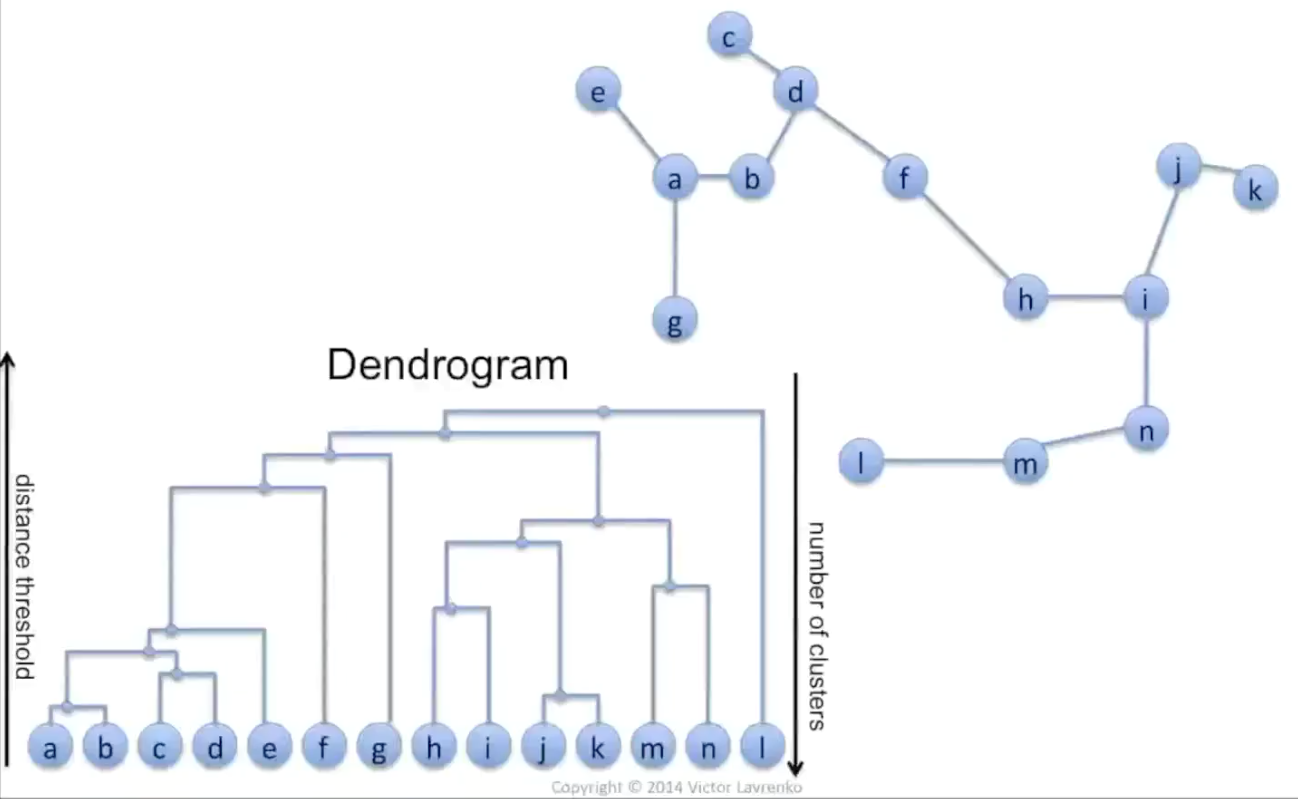
\includegraphics[width=0.8\textwidth]{assets/10_clustering}
\end{figure}

\subsubsection{Dendrogram}
\begin{figure}[H]
	\centering
	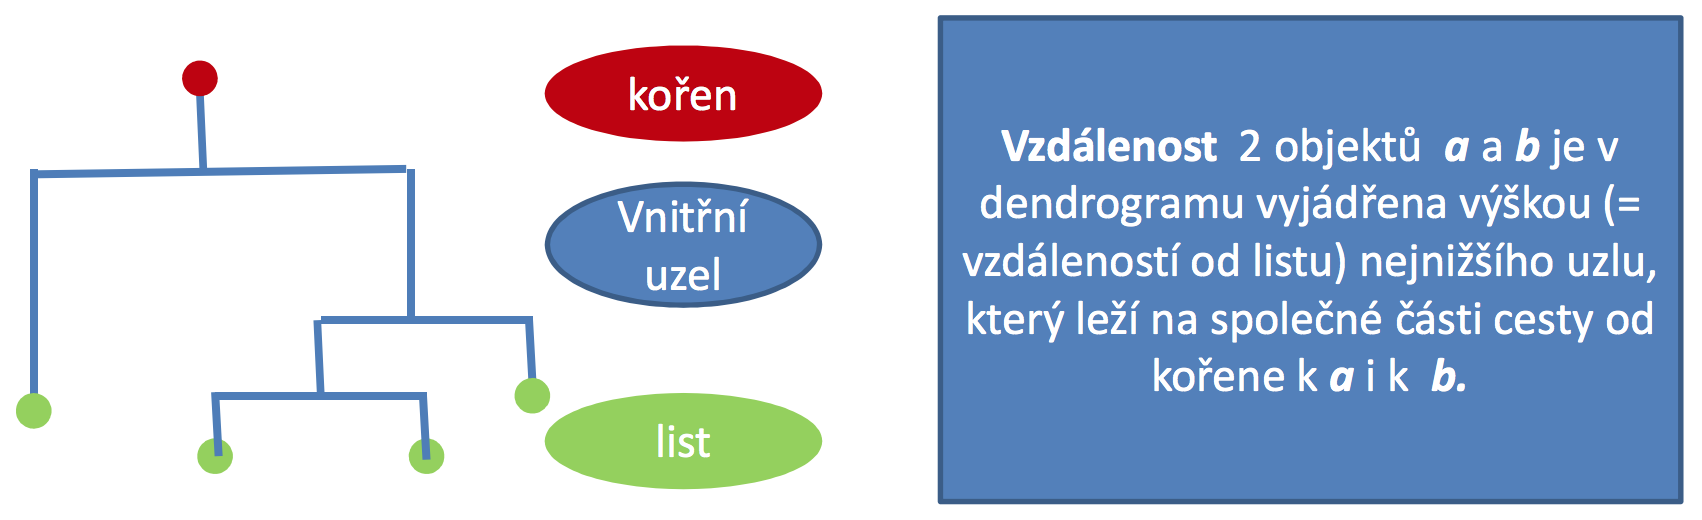
\includegraphics[width=0.8\textwidth]{assets/10_dendrogram}
\end{figure}

\subsubsection{Metody aglomerativního shlukování (měření vzdálenosti mezi shluky)}
Nevýhodou těchto metod je, že mohou vzniknout nejednoznačnosti už na začátku shlukování, které se projeví až později ve velkých shlucích. Předchozí kroky není možné změnit.
\begin{itemize}
\item \textbf{Single linkage} (nearest neighbor) -- vzdálenost shluků je určena vzdáleností \textbf{dvou nejbližších} prvků z různých shluků. Použití této metody vede k tomu, že jsou objekty taženy k sobě, výsledkem jsou dlouhé řetězy menších shluků.
\begin{figure}[H]
	\centering
	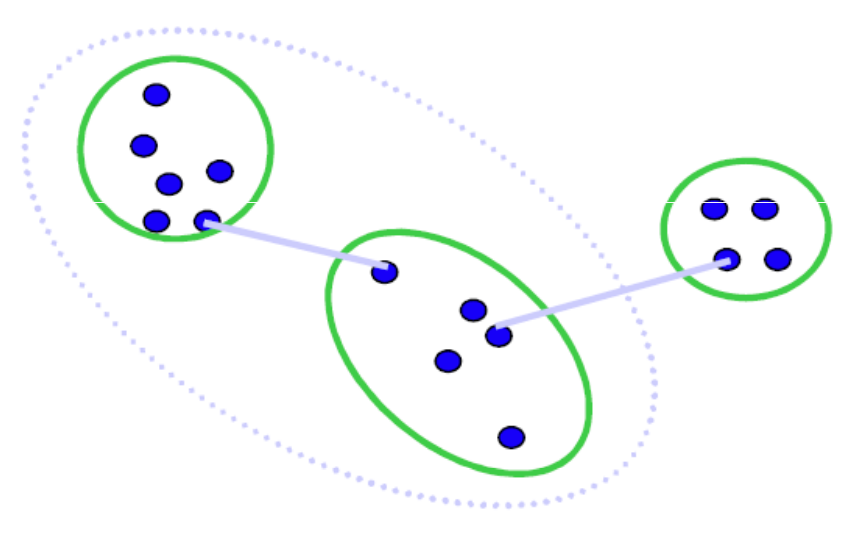
\includegraphics[width=0.3\textwidth]{assets/10_single_linkage}
\end{figure}
\item \textbf{Complete linkage} (furthest neighbor) -- vzdálenost shluků je určena naopak vzdáleností \textbf{dvou nejvzdálenějších} prvků z různých shluků. Funguje dobře, obvykle tvoří poměrně kompaktní shluky.
\begin{figure}[H]
	\centering
	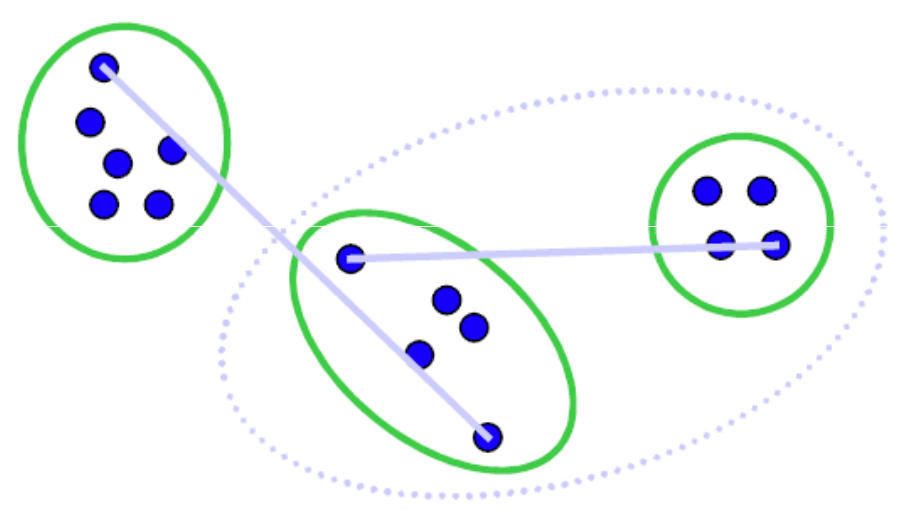
\includegraphics[width=0.3\textwidth]{assets/10_complete_linkage}
\end{figure}
\item \textbf{Average linkage} (průměrná vazba) -- vzdálenost shluků je určena jako \textbf{průměr vzdáleností všech párů objektů} z různých shluků. Může být ve \textbf{vážené} i \textbf{nevážené} podobě. Nejčastěji používaná míra pro vzdálenost.
\begin{figure}[H]
	\centering
	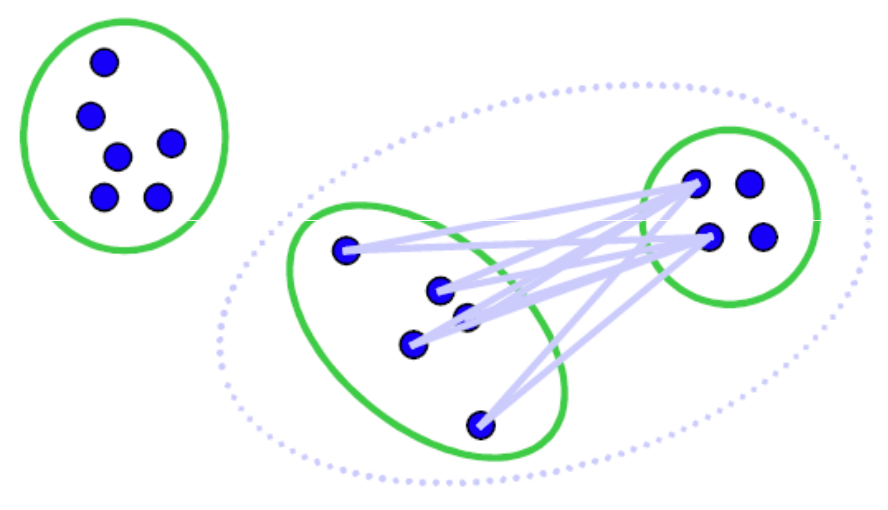
\includegraphics[width=0.3\textwidth]{assets/10_avg_linkage}
\end{figure}
\item \textbf{Centroidní metoda} -- pro spočítání nepodobnosti objektů se v této metodě využívá \textbf{euklidovská metrika}, v které se změří vzdálenosti \textbf{těžišť shluků} nebo objektů. Následně dojde ke sloučení shluků, které mají \textbf{nejmenší vzdálenost mezi těžišti}. Může být nevážená (mediánová metoda) nebo vážená (váží se podle velikosti shluku).
\item \textbf{Wardova metoda} -- metoda \textbf{založena na ztrátě informací}, která vzniká při shlukování. Kritériem pro shlukování je celkový součet druhých mocnin \textbf{odchylek} každého objektu od těžiště shluku, do kterého náleží.  Hodí pro práci s objekty, které mají stejný rozměr proměnných.
\end{itemize}

\subsubsection{Metody divizního shlukování}
Divizní metody berou množinu objektů, kterou mají zpracovat, jako \textbf{jeden shluk}, ten dále dělí na menší shluky a tím vytváří hierarchický systém. Každý shluk je rozdělen na dva nové, tak aby byl rozklad optimální vůči nějakému kritériu, a na konci tohoto postupu budou všechny shluky jednoprvkové. 

Tento postup je kvůli \textbf{exponenciální časové složitosti} (nalezení optimálního rozkladu množiny $n$ objektů vyžaduje prozkoumat až $2^{n-1}-1$ možností) prakticky proveditelný jen pro malý počet objektů.

\subsubsection*{MacNaughton–Smithova metoda}
Tato metoda se snaží \textbf{snížit časovou náročnost} divizních algoritmů až na \textbf{kvadratickou}, ale za cenu toho, že výsledné rozdělení \textbf{nemusí být optimální}. Je tedy aplikovatelná i na rozsáhlejší množiny objektů při nevelkých nárocích na čas počítače.

V porovnání s aglomerativními přístupy je ale \textbf{stále pomalejší}. Pomocí středních vzdáleností se vybere objekt uvnitř shluku, který vytvoří nový shluk a na základě rozdílů středních vzdáleností objektů z původního a objektů z nového shluku se objekt přiřadí do nového shluku, zůstane v původním. Výhodou oproti aglomerativnímu přístupu jsou j\textbf{ednoznačnější výsledky} pro větší shluky.

\subsection{Nehierarchické shlukování}
\begin{itemize}
\item Takový potup postup, při němž se každý objekt vloží do jednoho z $ k $ disjunktních shluků.
\item Předpokládá se, že uživatel předem stanoví $ k $, tj. požadovaný \textbf{cílový počet shluků}.
\end{itemize}

\subsubsection{K-means}
K-means \textbf{minimalizuje průměrnou vzdálenost mezi prvky} téhož shluku.
\begin{enumerate}
\item Stanov \textbf{požadovaný počet} $ k $ shluků.
\item Vyber náhodně výchozích $ k $ jader.
\item Přiřaď každému z N objektů číslo shluku, které odpovídá číslu \textbf{nejbližšího jádra}.
\item \textbf{Předefinuj pozice jader} všech k shluků tak, že bude použit \textbf{průměr hodnot} prvků v daném shluku.
\item Opakuj kroky 3. a 4. až do situace, kdy se příslušnost do shluků stabilizuje (po iteraci není žádný objekt zařazen do jiného shluku než před ní). 
\end{enumerate}

\begin{figure}[H]
	\centering
	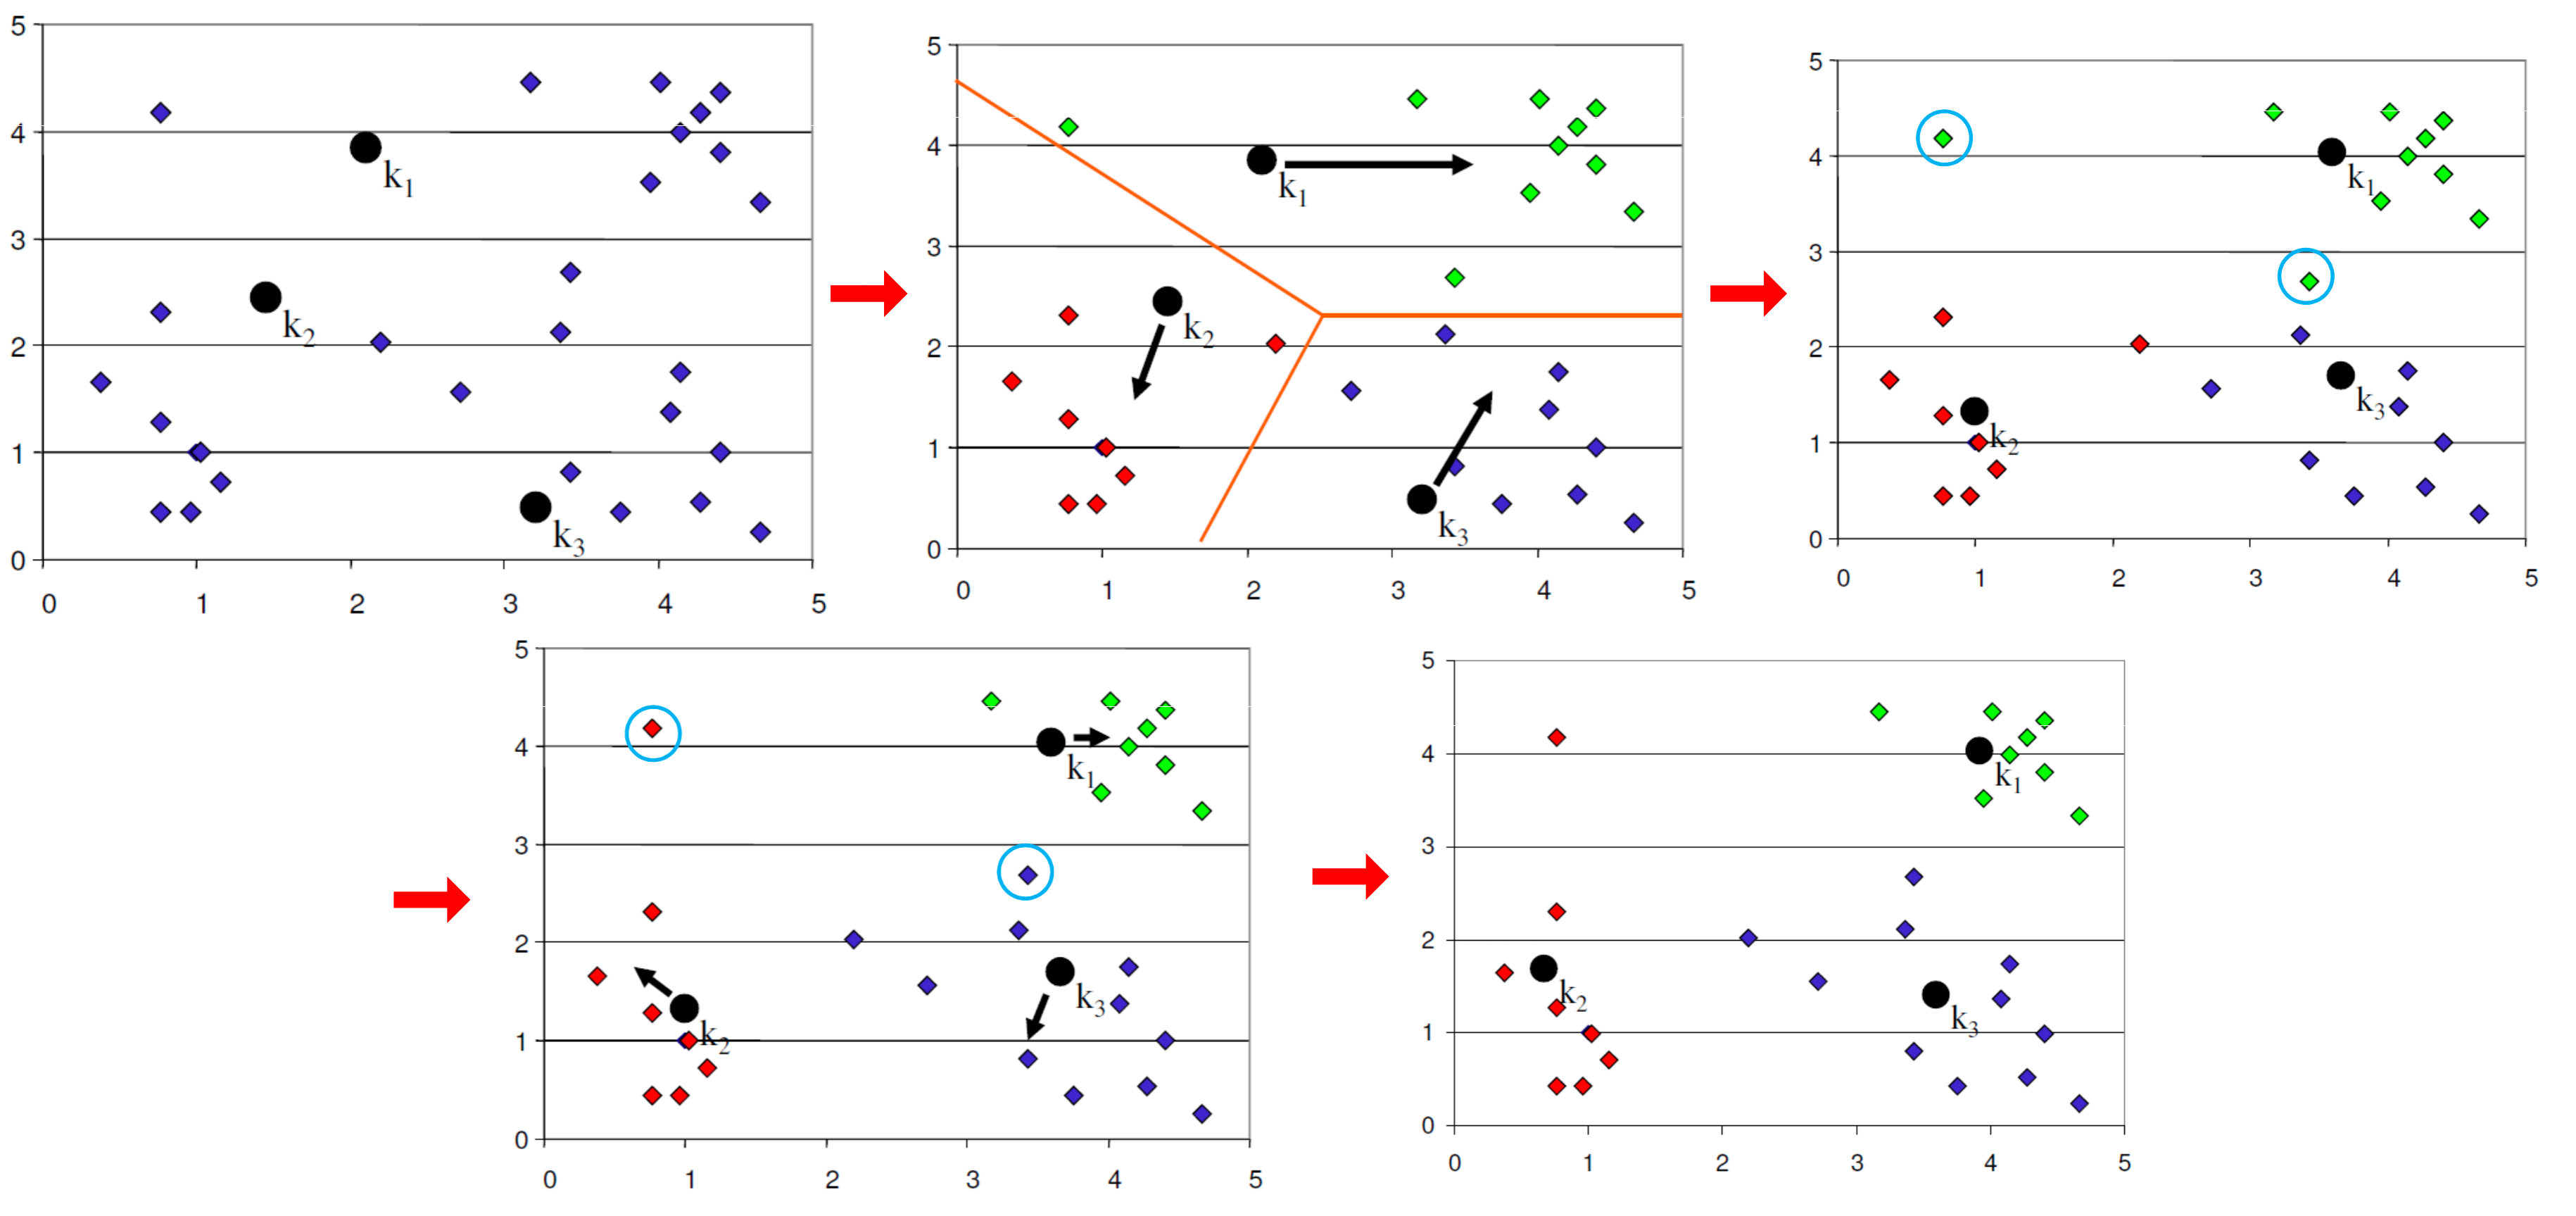
\includegraphics[width=\textwidth]{assets/10_kmeans}
\end{figure}

\noindent\textbf{Výhody}
\begin{itemize}
\item[$+$] \textbf{Jednoduchý} (lehká implementace i ladění).
\item[$+$] Intuitivní objektivní funkce, která optimalizuje podobnost uvnitř shluků.
\item[$+$] Poměrně \textbf{efektivní}: složitost $ O(T  K  m N) $, kde $ m $ je počet objektů, $ K $ je počet shluků, $ N $ počet atributů a $ T $ počet iterací. Obvykle bývají hodnoty $ T$ a $ K << m $ . 
\end{itemize}
\textbf{Nevýhody}
\begin{itemize}
\item[$-$] Použitelné, jen tam, kde \textbf{umíme spočítat průměr}. Co kategorická data?
\item[$-$] Velmi \textbf{záleží na inicializaci} – nebezpečí uvíznutí v lokálním minimu.
\item[$-$] \textbf{Požaduje} se znalost \textbf{počtu shluků}. 
\item[$-$] Nevhodné pro zašuměná data s výjimkami (outliers). 
\item[$-$] Nevhodné pro situace, kdy shluky nemají konvexní tvar .
\end{itemize}

\subsubsection{Odhad počtu shluků}
Sledujeme \textbf{jak rychle klesá} hodnota objektivní funkce (výpočet vzdálenosti) pro zvyšující se počet jader $ k $. Obecně hledáme ,,prudký pohyb'' v poklesu, který značí použití dané hodnoty $k$ (jakmile přestane $k$ prudce klesat, dosáhli jsme požadovaného počtu jader).